\documentclass[a4paper,12pt]{article}

\title{ CUDA task - report }
\author{ HPC | Aleksander Tudruj }
\date{ 2024-05-09 }

%\pagestyle {empty} %wyłącza numerowanie stron
\usepackage[super]{nth}

\usepackage[T1]{fontenc}
\usepackage[utf8]{inputenc}

\usepackage[usenames,dvipsnames]{xcolor}
\definecolor{Nblue}{RGB}{0, 72, 110}
\definecolor{Lblue}{RGB}{236, 250, 255}

\usepackage[headheight=0cm, left=1cm, right=1cm, top=2cm, bottom=2cm]{geometry}
\usepackage{amsfonts,amsmath}
\usepackage{amsmath,amsthm,amssymb}
\usepackage{gensymb}
\usepackage{enumitem}
\usepackage{stmaryrd}
\usepackage{blindtext}
\usepackage{hyperref}

\newcommand{\stirSet}[2]{\left\{\begin{array}{c}
                                    \!\!#1\\ \!\!#2
\end{array}\!\!\right\}}
\newcommand{\stirPerm}[2]{\left[\begin{array}{c}
                                    \!\!#1\\ \!\!#2
\end{array}\!\!\right]}
\newcommand{\stirBin}[2]{\left\left(\begin{array}{c}
                                        \!\!#1\\ \!\!#2
\end{array}\!\!\right\right)}
\newcommand{\set}[1]{\left\{ #1\right\}}
\newcommand{\floor}[1]{\lfloor #1\rfloor}
\newcommand{\ceil}[1]{\lceil #1\rceil}
\newcommand{\suma}[2]{\sum \limits_{#1}^{#2} }
\newcommand{\infsum}[1]{\sum_{#1}^{\infty}}
\newcommand{\mysuma}[2]{\sum_{#1}^{#2}}
\newcommand{\myroot}[2]{\sqrt[\leftroot{0}\uproot{0}#1]{#2}}

\newcommand{\vect}[1]{\overrightarrow{#1}}
\newcommand{\af}[1]{\text{af}{#1}}
\newcommand{\lin}[1]{\text{lin}{#1}}
\newcommand{\R}[0]{\mathbb{R}}
\newcommand{\C}[0]{\mathbb{C}}
\newcommand{\N}[0]{\mathbb{N}}
\newcommand{\Z}[0]{\mathbb{Z}}
\newcommand{\Q}[0]{\mathbb{Q}}
\newcommand{\mat}[1]{\left[\begin{matrix}
                               #1
\end{matrix}\right]}
\newcommand{\operacje}[1]{\begin{matrix}
                              #1
\end{matrix}}
\newcommand{\row}[0]{\text{R}}
\newcommand{\uklad}[1]{\begin{cases}
                           #1
\end{cases}}
\newcommand{\la}[0]{\left\left(}
\newcommand{\ra}[0]{\right\right)}

\newcommand{\myeq}[1]{\mathrel{\stackrel{\makebox[0pt]{\mbox{\normalfont\tiny #1}}}{=}}}

\usepackage { graphicx }

\usepackage{listings}
\usepackage{color}

\usepackage{multicol}

\definecolor{dkgreen}{rgb}{0,0.6,0}
\definecolor{gray}{rgb}{0.5,0.5,0.5}
\definecolor{mauve}{rgb}{0.58,0,0.82}

\lstset{frame=tb,
    language=C++,
    aboveskip=3mm,
    belowskip=3mm,
    showstringspaces=false,
    columns=flexible,
    basicstyle={\small\ttfamily},
    numbers=none,
    numberstyle=\tiny\color{gray},
    keywordstyle=\color{blue},
    commentstyle=\color{dkgreen},
    stringstyle=\color{mauve},
    breaklines=true,
    breakatwhitespace=true,
    tabsize=2
}

\usepackage{caption}
\usepackage{subcaption}


\newcommand{\plottimes}[4]{
    \begin{figure}
        \begin{subfigure}{.5\textwidth}
            \centering
            \includegraphics[width=.7\linewidth]{img/#1}
        \end{subfigure}%
        \begin{subfigure}{.5\textwidth}
            \centering
            \includegraphics[width=.7\linewidth]{img/#2}
        \end{subfigure}
        \begin{subfigure}{.5\textwidth}
            \centering
            \includegraphics[width=.7\linewidth]{img/#3}
        \end{subfigure}%
        \begin{subfigure}{.5\textwidth}
            \centering
            \includegraphics[width=.7\linewidth]{img/#4}
        \end{subfigure}
    \end{figure}
}

\begin{document}
    \maketitle

    \tableofcontents
    \newpage


    \section{Task approach}

    The task was to implement a indexer and query engine for biological variance search.
    The indexing is done purely on the CPU, while the query engine has multiple implementations.
    This report will focus on comparing the performance of the CPU and GPU implementations of the query engine.

    Both CPU and GPU approaches has multiple strategies. Some of them are still
    available in the code, but are not used in the final implementation.
    Some implementations regarding the GPU were modifications of the existing code.
    Code is structured into multiple files and two modules responsible for indexing and querying.
    They share a common set of structures and functions.


    \section{Indexer}
    Indexing is fairly simple. The input is a file with each line containing tab separated values.
    First columns, namely CHROM, POS, REF, ALT, are used to create a key.
    Considering the VCF file format, the key is unique for each record.

    The index key is a uint64\_t value, where first
    5 bits are for the chromosome, next 55 bits are for the position,
    and the last 4 bits are for ref and alt, each taking 2 bits.

    Such approach is sufficient, as the chromosome can be a number from 1 to 22, X, Y or M.
    Letters are mapped to numbers, so we can have up to 25 chromosomes, thus 5 bits are enough.
    Both ref and alt can be one of 4 letters, A, C, G, T, so 2 bits are enough for each.

    The order of values in the key is important, as we want to sort the indexes by chromosome, position, ref and alt.
    Sorted index can be used to speed up the query engine.
    This is based on a fact, that bitwise lexicographical comparison of the keys is the same as comparison of the values.

    First indexing strategy was to create a structure that holds the key and the offset in the input file.
    This proved to be inefficient, as the structure was too big and could not be easily compared.
    Using uint64\_t as index is both efficient and simple.
    What is more, it does not require to decode once coded key.

    According to the documentation the input file is sorted by CHROM and POS.
    Assuming there are no duplicate keys, the indexer can simply read the input file line by line,
    sort up to 16 different values of REF and ALT, and write the key to the output file.

    Each index key has a corresponding offset in the input file.
    The line starts at the offset and ends at the next newline character.
    The original database is appended at the end of the index file,
    so the offset can be used to read the record from the database.


    \section{Query engine}

    We the indexing done, we can now implement the query engine.
    The query engine is responsible for finding all the records that match the query.
    The query is a simple structure, containing the same fields as the index, again coded
    as a uint64\_t value.
    Matching index to query is done by chromosome, position, ref and alt.
    The offset is the value that we are interested in, as it points to the record in the database.

    Querying is structured the same way regardless the chosen strategy.
    First we read the indexes from the index file.
    Then we read a batch of queries from the query file.
    The batch is then processed using selected strategy and the results
    are stored in an array of indexes. At the end IO thread writes the results to the output file
    based on the indexes of the offsets. Querying is done on uint64\_t indexes,
    and the values are based on the index in the index array. At the end we write the results to the output file,
    based on the database offsets.

    \begin{center}
        \begin{tabular}{||c || c | c||}
            \hline
            Id       & Key (CHROM + POS + REF + ALT) & Value (Offset) \\
            \hline
            usize    & uint64                        & uint64         \\
            \hline\hline
            0        & 0xb0000000110600ee            & 3857563        \\
            1        & 0x200000004ed07851            & 4829911        \\
            2        & 0x800000002509ff83            & 4829911        \\
            $\vdots$ & $\vdots$                      & $\vdots$       \\
            \hline
        \end{tabular}
    \end{center}

    The above table shows example of the index file.
    Query contains values referencing Key column, and query engine is responsible for finding the corresponding Value,
    by matching the Key to the on Id in the array.

    \begin{center}
        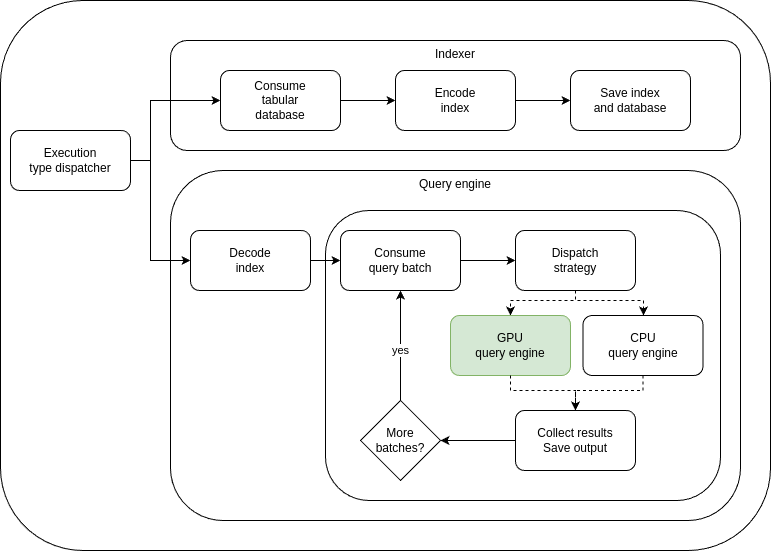
\includegraphics[width=0.75\linewidth]{img/HPC-Cuda}
    \end{center}

    The above diagram shows the structure of the query engine.

    \subsection{Strategies}

    \subsubsection{Single core, linear CPU implementation}

    Although the CPU implementation is not the most efficient, it is the simplest to implement.
    This can be used to compare the performance of the GPU implementation.
    First, trivial implementation is done, where we iterate over all the indexes and compare them to the query.
    Let $q$ be the number of queries, and $n$ be the number of indexes.
    The complexity of this implementation is $O(n q)$.
    Once the resulting offsets are found, we can read the records from the database and
    dump them to the output file.

    \subsubsection{Single core, binary CPU implementation}

    The above implementation can be improved by sorting the indexes.
    The indexer can be modified to sort the indexes by position, chromosome, ref and alt.
    The input database is sorted on first two columns, namely CHROM and POS.
    The rest of the columns, namely REF and ALT, can take up to 16 different values,
    thus indexer can easily sort the indexes by these columns in constant time.
    Once the indexer sorted the indexes, the query engine can use binary search to find the matching indexes.
    Considering the same $q$ and $n$ as above, the complexity of this implementation is $O(n + q \log n)$.

    \subsubsection{Single core, binary CPU with oneway jumping}

    This approach is similar to the previous one, but instead of using binary search, we use oneway jumping.
    We start at index 0, and try to jump over by a big step which is a power of 2.
    If the key at the new index is smaller than the query, we jump again.
    If the key is bigger, we start binary search between the previous and current index.
    This approach can be faster when implementing on GPU, as it contains less branching in code.

    \subsubsection{Multi core, linear CPU implementation}

    The CPU implementation can be parallelized by using multiple threads using OpenMP.
    In order to keep track of the results, we reserve a vector of results for each query.

    \subsubsection{Multi core, binary CPU implementation}

    Similar to the single core binary implementation, we can parallelize the binary search.

    \subsubsection{Multi core, binary CPU with oneway jumping}

    Similar to the single core oneway jumping implementation, we can parallelize the oneway jumping.

    \subsubsection{GPU implementation, linear}

    The GPU implementation is based on the linear CPU implementation.

    The indexes are copied to the GPU memory, and the queries are copied to the GPU memory.
    The kernel is launched with the indexes and queries as arguments.
    The kernel iterates over all the indexes and compares them to the query.
    The results are stored in the GPU memory.
    Once the kernel finishes, the results are copied back to the CPU memory.

    \subsubsection{GPU implementation, binary}

    The GPU implementation is based on the binary CPU implementation.

    Everything is the same as in the linear GPU implementation, except the kernel uses binary search to find the matching indexes.

    \subsubsection{GPU implementation, oneway jumping}

    The GPU implementation is based on the oneway jumping CPU implementation.

    Everything is the same as in the linear GPU implementation, except the kernel uses oneway jumping to find the matching indexes.

    \subsection{Strategies comparison}

    Empirical tests were done to compare the performance of the strategies.
    Tests were run on entropy cluster, using the provided database and randomly generated queries of multiple sizes.

    The results can be seen in the diagrams \ref{fig:sub1} and \ref{fig:sub2}.

    \begin{figure}[h]
        \begin{subfigure}{.5\textwidth}
            \centering
            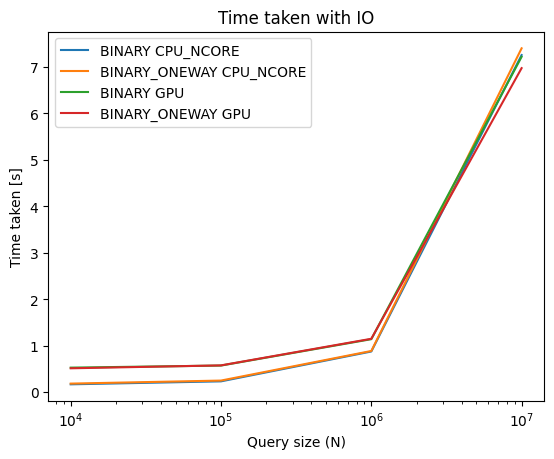
\includegraphics[width=.8\linewidth]{img/time_N_total_time}
            \caption{Total execution time}
            \label{fig:sub1}
        \end{subfigure}%
        \begin{subfigure}{.5\textwidth}
            \centering
            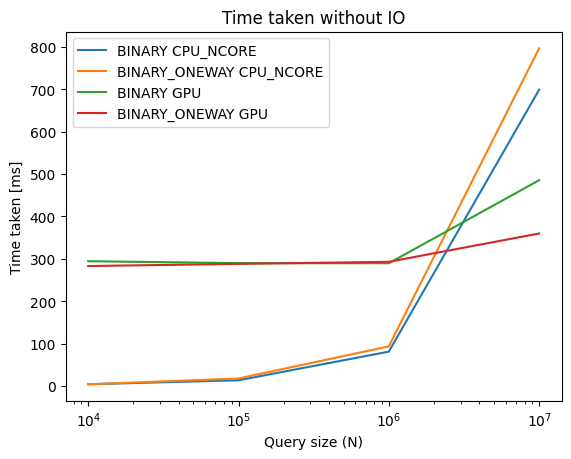
\includegraphics[width=.8\linewidth]{img/time_N_query_time}
            \caption{Query execution time}
            \label{fig:sub2}
        \end{subfigure}
        \caption{Comparison of the strategies}
        \label{fig:test}
    \end{figure}

    It can be clearly seen that most part of the task is IO,
    so the performance tuning focus was on the query execution time.
    None of the tests include linear strategy, as it is the slowest and not worth comparing.

    For big enough queries, the GPU implementation is the fastest.
    According to the tests, the oneway jumping strategy is the fastest.

    There were many tries to optimize the GPU implementation, but the results were not satisfying.
    One of them was to run smaller number of groups, but resolve multiple queries in one thread.
    Another was to use shared memory, but binary search jumps are unpredictable, so it was not possible to use it efficiently.

    More detailed times can be found in the at the end of the report.

    \subsection{Conclusions}

    Implementing the query engine on the GPU is a good idea, as it can be faster than the CPU implementation for big enough queries.
    The biggest bottleneck is the IO, as scanning the index if much faster than producing the output file.
    We can try to implement query engine, that reads part of the query, runs it, and writes the results to the output file, while
    performing the next query, but query is incomparably faster than the IO.


    \section{Detailed times}

    \plottimes{time_bar_N10000_total_time}{time_bar_N10000_query_time}{time_boxplot_N10000_total_time}{time_boxplot_N10000_query_time}
    \plottimes{time_bar_N100000_total_time}{time_bar_N100000_query_time}{time_boxplot_N100000_total_time}{time_boxplot_N100000_query_time}
    \plottimes{time_bar_N1000000_total_time}{time_bar_N1000000_query_time}{time_boxplot_N1000000_total_time}{time_boxplot_N1000000_query_time}
    \plottimes{time_bar_N10000000_total_time}{time_bar_N10000000_query_time}{time_boxplot_N10000000_total_time}{time_boxplot_N10000000_query_time}

\end{document}
